% sezione 5
\section{VarNet: Variant Convolutional Neural Network}
\begin{table}[htbp]
	\centering
	\caption{Tabella del training GPU si dataset oversampled di VarNet}
	\begin{tabular}{cccc}
		\toprule
		Fold ID & Accuracy & Epoche & Tempo \\
		\midrule
		      0 & 94\% & 200 & 14:00:34 \\
            1 & 95\% & 200 & 14:05:03 \\
            2 & 95\% & 189 & 13:22:22 \\
            3 & 95\% & 200 & 14:06:19 \\
            4 & 95\% & 200 & 14:06:19 \\
            5 & 95\% & 200 & 14:06:44 \\
            6 & 93\% & 200 & 14:06:45 \\
            7 & 95\% & 200 & 14:07:14 \\
            8 & 95\% & 200 & 14:07:05 \\
            9 & 96\% & 200 & 14:07:50 \\
		\bottomrule
	\end{tabular}
	\label{table:GPU-varnet}
\end{table}

\begin{table}[htbp]
	\centering
	\caption{Tabella del training GPU si dataset oversampled di Net}
	\begin{tabular}{cccc}
		\toprule
		Fold ID & Accuracy & Epoche & Tempo \\
		\midrule
		0 & 94\% & 44 & 2:40:24 \\
            1 & 95\% & 131 & 8:00:44 \\
            2 & 95\% & 49 & 2:56:24 \\
            3 & 95\% & 50 & 3:00:12 \\
            4 & 95\% & 200 & 12:10:15 \\
            5 & 94\% & 200 & 12:00:00 \\
            6 & 94\% & 43 & 2:34:48 \\
            7 & 95\% & 49 & 2:57:09 \\
            8 & 95\% & 39 & 2:21:24 \\
            9 & 96\% & 51 & 2:30:36 \\
		\bottomrule
	\end{tabular}
	\label{table:GPU-Net}
\end{table}
\label{sec:varnet}
In questa sezione mostriamo l'applicazione del workflow che ha portato alla progettazione di VarNet ed il suo confronto
con Net. In primo luogo descriviamo VarNet nel suo complesso. Dopodiché mostriamo i risultati della rete e le sue
differenze con Net nei punti fondamentali del progetto: classificazione, interpretabilità delle decisioni prese in 
base al task assegnato e validazione dei biomarker estratti.
% 5.1
\subsection{VarNet vs Net: Less is more?}
Nella seguente sezione spieghiamo come viene organizzata e strutturata la rete VarNet. Dapprima mostriamo quali sono i
goal interessati dallo sviluppo di VarNet, poi estraiamo le ipotesi di base che servono alla rete per
raggiungere tali scopi, infine mostriamo come vengono effettuate le principali modifiche che hanno portato alla nascita
di VarNet.

% 5.1.1 
\subsubsection{Assunzioni e Obiettivi VarNet}
Analizzando la metodologia applicata alla rete CNN di riferimento (per ulteriori dettagli consultare la sezione
\ref{methology_sec:ClassNN}) ed i risultati ottenuti sulla pipeline dell'intero progetto (cfr. \ref{sec:result})
ci siamo posti la seguente domanda:
\begin{quote}
    Quali sono i punti salienti che possono rendere l'individuazione dei biomarker più efficiente, affidabile e veloce? 
\end{quote}
Da questa domanda sono stati estratti, usando la notazione espressa nella sezione \ref{appendix}, i moduli che offrivano
i migliori servizi per raggiungere tale scopo, raggruppati in 2 macro-categorie legate al processo di sviluppo di un
progetto che usa il Deep Learning:
\begin{enumerate}
    \item \textbf{Dati Genomici:} di questa categoria fanno parte i moduli \texttt{Raw Data}, \texttt{Preprocessing} e
    \texttt{Biological Validation}. Questi si occupano di trattare i \textit{gene expression data}, che rappresentano 
    il dominio di applicazione del nostro problema. Si potrebbe, quindi, pensare di migliorarne le qualità o 
    cambiare il metodo con cui vengono validati i risultati biologici ottenuti dal modello, oppure si potrebbero
    utilizzare diversi progetti di raccolta ed analisi di ulteriori campioni biologici ampliando la conoscenza di
    FireHose. La complessità di tale operazioni può essere demandata ad ulteriori indagini e quindi tale categoria 
    non sarà scelta per raggiungere lo scopo espresso in precedenza.
    %
    \item \textbf{Modello Deep Learning:} in questa categoria ci sono i moduli \texttt{Training \& Test},
    \texttt{Heatmaps Generation} e \texttt{Performance Evaluation}. Essi trattano tutti gli aspetti fondamentali per 
    il modello di Deep Learning scelto (cfr. \ref{subsubsec:3.4.1}), dall'addestramento della rete alla sua valutazione
    ed interpretabilità decisionale. 
\end{enumerate}

Da quanto espresso in precedenza abbiamo deciso di concentrare i nostri sforzi sul modello DL usato nel lavoro di Lyu e
Haque \cite{lyu2018deep}, concentrandoci sui seguenti due punti:
\begin{enumerate}
    \item \textbf{Architettura:} la composizione degli strati nascosti della rete rappresenta il primo punto focale 
    che ci permette di migliorare le performance del modello.
    \item \textbf{Learning Blocks:} li definiamo come i componenti fondamentali che modellano tutti gli aspetti 
    dell'apprendimento necessari all'efficacia della rete feedforward. Essi sono: \textit{Activation Function},
    \textit{Loss Function} e \textit{Optimizer}. 
\end{enumerate}
% 5.1.2
\subsubsection{Schema della rete: VarNet vs Net}
La Figura \ref{fig:varnet-structure} mostra l'architettura di VarNet, confrontandola con Net (Figura \ref{fig:cnn} a
pagina \pageref{fig:cnn}) la prima differenza notabile è che VarNet contiene un livello di profondità in più 
osservando le dovute precauzioni sul dataset (cfr \ref{methology_sec:ClassNN}). 
In VarNet, dunque, viene aggiunto prima del layer di drop-out un quarto layer
convoluzionale "conv4" contenente 512 filtri e posti immediatamente dopo di esso, un layer di Max-Pooling e Batch
Normalization. Oltre ciò cambiano le dimensioni del primo layer fully-connected che risulta essere di 18432. Il resto
delle rete è fatta come Net. Una seconda differenza tra le reti è basata sul numero di parametri e dal peso complessivo
occupato sul disco: NET: Total-params: $38,778,755$, Total-Size (MB): $160.65$ e VARNET: Total-params: $17,415,555$,
Total-Size (MB): $80.78$. 
Concludiamo dicendo che la modifica è stata indotta dalla parziale applicazione del principio fondamentale dietro il
design di VGG \cite{simonyan2014very}, cercando di sfruttare il numero di filtri, andando ad aumentare la profondità dei
livelli in cui ci sono i layer convoluzionali e cercando di mitigare il problema di rendere meno time-consuming il
modello.
\begin{figure}[h!]
		\centering
		\includesvg[inkscapelatex=false, width=\textwidth]{images/VarNet}
  		\caption{Composizione della Rete VarNet}
        \label{fig:varnet-structure}
\end{figure}
% 5.1.3
\subsubsection{Learning blocks: VarNet vs Net}
Illustriamo ora le differenze tra le reti nei rispettivi learning blocks precedentemente definiti:
\begin{description}
 \item[Activation Function:] Per cercare di risolvere il problema di ReLU (cfr. \ref{subsubsec:act_func}), viene scelta
    come alternativa SeLU (Scaled Exponential Linear Units) che è una funzione di attivazione che induce 
    l'auto-normalizzazione. Le attivazioni delle reti neurali che usano SELU convergono automaticamente a una media 
    zero e ad una varianza unitaria. La SeLU e descritta come segue:
 \begin{equation}
    f(x) = \lambda x \ \ \ \ \ \ \ \text{if} \ \ x > 0 
    f(x)= \lambda \alpha (e^x - 1) \ \ \ \ \ \ \ \text{if} \ \ x \leq 0 
\end{equation}
I principali vantaggi sono: (1) SeLU non avrà il problema di retropropagare gradienti molto piccoli. (2) SeLU non soffre
di momenti inattivi o morti. 
Uno svantaggio è che esistono pochi research paper che mostrano risultati efficienti di SeLU su diverse architetture.

 \item[Loss Function:] Per sopperire alla mancanza della Cross-Entropy (cfr. \ref{subsubsec:loss}) viene utilizzata la
    Multi Margin Loss che può essere intesa come il tentativo di assicurarsi che il punteggio per la classe corretta sia
    superiore alle altre classi di almeno un certo margine $\delta > 0$, altrimenti si incorre in una perdita che
    comporta una penalità al modello.
 
 \item[Optimizer:] Si usa Nadam, che combina Adam con NAG (Nesterov Accelerated Gradient che è un ottimizzatore SGD
    basato sulla quantità di moto che "guarda avanti" a dove i saranno parametri, per calcolare il gradiente ex post
    piuttosto che ex ante), e che rispetto ad Adam risulta essere migliore nei task di ottimizzazione. 
\end{description}

% 5.1.4 
\subsubsection{Risultati training: VarNet vs Net}
Osservando le Tabelle \ref{table:GPU-varnet} a pagina \pageref{table:GPU-varnet} e \ref{table:GPU-Net} a 
pagina \pageref{table:GPU-Net} si può fare la seguente osservazione: a parità
prestazionali di GPU si nota che il numero di epoche ed i tempi su singola fold di VarNet sono più alti di Net. 
Questo è dovuto alla ridotta \textbf{batch size} rispetto a quella di Lyu e Haque \cite{lyu2018deep} dovuta alla
scarsità di memoria disponibile per la GPU in uso. Oltre ciò, la causa si addurre anche a come i learning blocks di
VarNet suppongano principalmente che la sua loss function sia influenzata maggiormente dalla dispersività dei dati,
usati in numero ridotto nel lotto impiegato per la fase di training (cfr. \ref{subsubsec:optimizer}). 

% 5.2 
\subsection{Valutazione Classificazione}
\label{subsec:class-val-varnet}
Dalla matrice di confusione si può notare che la maggior parte delle classi sono classificate correttamente, tuttavia 
ci sono alcune classificazioni errate: 
\begin{enumerate}
    \item I campioni READ sono stati per lo più erroneamente classificati in COAD e ciò
          potrebbe essere dovuto ai pochi campioni di READ rispetto a quelli di COAD;
    \item alcuni campioni di ESCA ($25\%$) sono classificati erroneamente come STAD, questo potrebbe essere causato da
          alcuni campioni di ESCA i quali rientrano nella tipologia tumorale di carcinoma e che vengono visti dal
          modello come adenocarcinomi\footnote{La principale differenza tra le due tipologie e la seguente: 
          il carcinoma è un tumore maligno (cancro) che prende origine dalle cellule che compongono il tessuto
          epiteliale mentre l'adenocarcinoma è un tumore maligno (cancro) che prende origine dalle cellule che
          compongono un tipo di tessuto epiteliale specifico, ossia quello ghiandolare. L’adenocarcinoma, in sintesi, 
          è un tipo di carcinoma.}. Ciò avviene perché la forma di adenocarcinoma si è presentata con una frequenza
          maggiore nei campioni ESCA rispetto alla sua forma di carcinoma dato che i campioni raccolti dal progetto
          FireHose provengono dagli Stati Uniti e questa forma per ESCA risulta essere la più vista nella sua
          popolazione;
    \item alcuni campioni di UCS ($33,33\%$) sono classificati erroneamente come UCEC e ciò può essere causato dalla 
          difficoltà del modello a discriminare correttamente una particolare caratteristica che emerge nei campioni
          UCS: essi sono legati ad un tipologia particolare di cancro cioè il carcinosarcoma, questo significa, 
          in ambito biologico, che osservando i campioni di tale coorte tumorale al microscopio si vede che a 
          livello di proprietà istologiche, essi mostrano caratteristiche sia del tumore carcinoma endometriale sia 
          del sarcoma. Per cui in alcuni campioni questa manifestazione è avvenuta in maniera sbilanciata facendo
          generare l'errore di classificazione con la coorte UCEC che è un sotto-tipologia di carcinoma specifico 
          della zona endometriale dell'utero.
\end{enumerate}

\begin{figure}[h!]
    \centering
    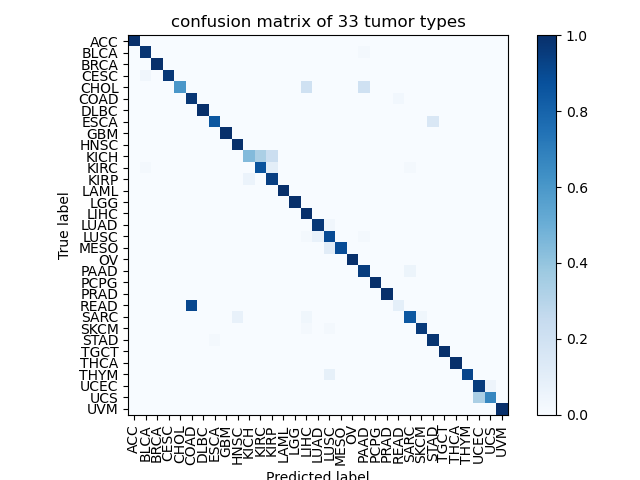
\includegraphics[width=0.6\textwidth]{images/cnfMatrices/cnf_matrix_varnet.png}
    \caption{Confusion Matrix di VarNet}
    \label{fig:cnf_matrix_varnet}
\end{figure}

% Tabella - [VarNet] Performance Generali
\begin{table}[h!]
    \centering
    \caption{Performance del metodo utilizzato con VarNet}
    \begin{tabular}{crrrr}
        \toprule
         Metodo & Accuracy & Precision & Recall & F1-score \\
         \midrule
         CNN    & 94.83\%    & 94.66\%     & 94.83\%  & 94.45\%     \\
         \bottomrule
    \end{tabular}
    \label{tab:method_score_VarNet}
\end{table}

% Tabella: [Caso Generale] Accuracy per coorte tumorale
\begin{table}[h!]
    \centering 
    \caption{Accuracy per coorte tumorale (calcolo effettuato su CPU e su dataset senza oversampling).}
    \large{
    \begin{tabular}{lrrr}
    \toprule
     Coorte  & Accuratezza & Accuratezza & Accuratezza \\
             & ns. metodo  & Variante    & Riferimento \\
    \midrule
     ACC  & \textbf{1.00} & \textbf{1.00} & 0.95 \\
     BLCA &  0.98 & 0.98 & 0.97 \\
     BRCA &  0.99 & 0.99 & 0.99 \\
     CESC &  \textbf{0.97} & \textbf{0.97} & 0.93 \\
     CHOL &  \textbf{1.00} & \textbf{0.80} & 0.56 \\
     COAD &  0.97 & 0.97 & 0.95 \\
     DLBC &  1.00 & 1.00 & 1.00 \\
     ESCA &  \textcolor{blue}{0.70} & 0.75 & 0.77 \\
     GBM  &  0.94 & 0.94 & 0.94 \\
     HNSC &  0.98 & 0.98 & 0.98 \\
     KICH &  \textbf{0.89} & \textbf{0.89} & 0.87 \\
     KIRC &  0.97 & 0.97 & 0.95 \\
     KIRP &  \textcolor{blue}{0.88} & \textcolor{blue}{0.88} & 0.93 \\
     LAML &  1.00 & 1.00 & 1.00 \\
     LGG  &  1.00 & 1.00 & 0.98 \\
     LIHC &  0.95 & 0.95 & 0.97 \\
     LUAD &  \textcolor{blue}{0.91} & \textcolor{blue}{0.91} & 0.95 \\
     LUSC &  0.91 & \textcolor{blue}{0.89} & 0.91 \\
     MESO &  \textbf{0.89} & \textbf{0.89} & 0.94 \\
     OV   &  1.00 & 1.00 & 0.99 \\
     PAAD &  0.95 & 0.95 & 0.97 \\
     PCPG &  1.00 & 1.00 & 1.00 \\
     PRAD &  1.00 & 1.00 & 1.00 \\
     READ &  \textcolor{blue}{\textbf{0.09}} & \textcolor{blue}{\textbf{0.09}} & 0.35 \\ 
     SARC &  1.00 & 1.00 & 0.97 \\ 
     SKCM &  1.00 & 1.00 & 0.98 \\ 
     STAD &  0.96 & 0.96 & 0.96 \\ 
     TGCT &  1.00 & 1.00 & 0.99 \\ 
     THCA &  1.00 & 1.00 & 1.00 \\ 
     THYM &  1.00 & 1.00 & 0.99 \\ 
     UCEC &  1.00 & 1.00 & 0.96 \\ 
     UCS  &  \textcolor{blue}{0.67} & \textcolor{blue}{0.67} & 0.81 \\ 
     UVM  &  1.00 & 1.00 & 0.99 \\ 
    \bottomrule
    \label{tab:CPU-res}
    \end{tabular} 
    } %end large
\end{table}


\subsection{Heatmap Generation}
	\begin{figure}[h!]
		\centering
		% prima riga
		\subfloat[][]{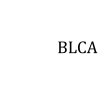
\includegraphics[scale=0.7]{images/heatmapsVarNet/BLCATitle}} \hfill
		\subfloat[][]{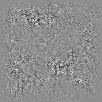
\includegraphics[scale=0.7]{images/heatmapsVarNet/BLCAggcamFold0}} \hfill % 1
		\subfloat[][]{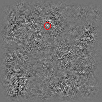
\includegraphics[scale=0.7]{images/heatmapsVarNet/BLCAggcamFold1}} \hfill % 2
		\subfloat[][]{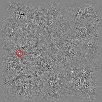
\includegraphics[scale=0.7]{images/heatmapsVarNet/BLCAggcamFold2}} \hfill % 3
		\subfloat[][]{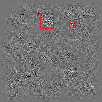
\includegraphics[scale=0.7]{images/heatmapsVarNet/BLCAggcamFold3}} \hfill % 4
		\subfloat[][]{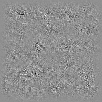
\includegraphics[scale=0.7]{images/heatmapsVarNet/BLCAggcamFold4}} \hfill % 5
		\subfloat[][]{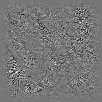
\includegraphics[scale=0.7]{images/heatmapsVarNet/BLCAggcamFold5}} \hfill % 6
		\subfloat[][]{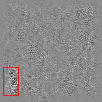
\includegraphics[scale=0.7]{images/heatmapsVarNet/BLCAggcamFold6}} \hfill % 7
		\subfloat[][]{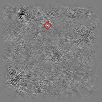
\includegraphics[scale=0.7]{images/heatmapsVarNet/BLCAggcamFold7}} \hfill % 8
		\subfloat[][]{
\includegraphics[scale=0.7]{images/heatmapsVarNet/BLCAggcamFold8}} \hfill % 9
		\subfloat[][]{
\includegraphics[scale=0.7]{images/heatmapsVarNet/BLCAggcamFold9}} \\     % 10
	   \vspace{-8mm}
		% seconda riga
		\subfloat[][]{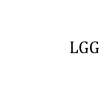
\includegraphics[scale=0.7]{images/heatmapsVarNet/LGGTitle}} \hfill
		\subfloat[][]{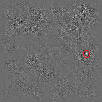
\includegraphics[scale=0.7]{images/heatmapsVarNet/LGGggcamFold0}} \hfill % 11
		\subfloat[][]{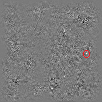
\includegraphics[scale=0.7]{images/heatmapsVarNet/LGGggcamFold1}} \hfill % 12
		\subfloat[][]{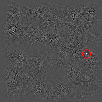
\includegraphics[scale=0.7]{images/heatmapsVarNet/LGGggcamFold2}} \hfill % 13
		\subfloat[][]{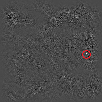
\includegraphics[scale=0.7]{images/heatmapsVarNet/LGGggcamFold3}} \hfill % 14
		\subfloat[][]{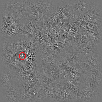
\includegraphics[scale=0.7]{images/heatmapsVarNet/LGGggcamFold4}} \hfill % 15
		\subfloat[][]{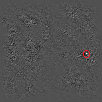
\includegraphics[scale=0.7]{images/heatmapsVarNet/LGGggcamFold5}} \hfill % 16
		\subfloat[][]{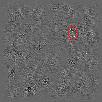
\includegraphics[scale=0.7]{images/heatmapsVarNet/LGGggcamFold6}} \hfill % 17
		\subfloat[][]{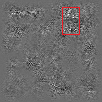
\includegraphics[scale=0.7]{images/heatmapsVarNet/LGGggcamFold7}} \hfill % 18
		\subfloat[][]{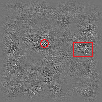
\includegraphics[scale=0.7]{images/heatmapsVarNet/LGGggcamFold8}} \hfill % 19
		\subfloat[][]{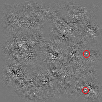
\includegraphics[scale=0.7]{images/heatmapsVarNet/LGGggcamFold9}} \\     % 20
		\vspace{-8mm}
		% terza riga
		\subfloat[][]{
\includegraphics[scale=0.7]{images/heatmapsVarNet/PRADTitle}} \hfill
		\subfloat[][]{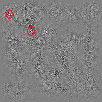
\includegraphics[scale=0.7]{images/heatmapsVarNet/PRADggcamFold0}} \hfill % 21
		\subfloat[][]{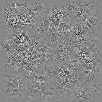
\includegraphics[scale=0.7]{images/heatmapsVarNet/PRADggcamFold1}} \hfill % 22
		\subfloat[][]{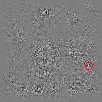
\includegraphics[scale=0.7]{images/heatmapsVarNet/PRADggcamFold2}} \hfill % 23
		\subfloat[][]{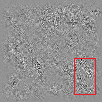
\includegraphics[scale=0.7]{images/heatmapsVarNet/PRADggcamFold3}} \hfill % 24
		\subfloat[][]{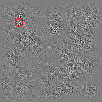
\includegraphics[scale=0.7]{images/heatmapsVarNet/PRADggcamFold4}} \hfill % 25
		\subfloat[][]{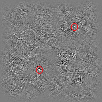
\includegraphics[scale=0.7]{images/heatmapsVarNet/PRADggcamFold5}} \hfill % 26
		\subfloat[][]{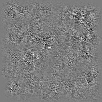
\includegraphics[scale=0.7]{images/heatmapsVarNet/PRADggcamFold6}} \hfill % 27
		\subfloat[][]{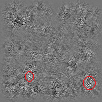
\includegraphics[scale=0.7]{images/heatmapsVarNet/PRADggcamFold7}} \hfill % 28
		\subfloat[][]{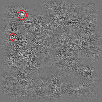
\includegraphics[scale=0.7]{images/heatmapsVarNet/PRADggcamFold8}} \hfill % 29
		\subfloat[][]{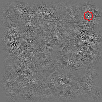
\includegraphics[scale=0.7]{images/heatmapsVarNet/PRADggcamFold9}} \hfill % 30
		\caption{Alcuni esempi di heatmap legate a VarNet. Ogni colonna rappresenta il risultato di una fold. Nella prima riga ci sono le heatmap %
					del tipo di tumore BLCA, nella seconda di LGG e nella terza di PRAD.}
		\label{fig:esempi-heatmap-varnet}
	\end{figure}
Confrontando le Figure \ref{fig:esempi-heatmap-varnet} a pagina \pageref{fig:esempi-heatmap-varnet} e 
\ref{fig:esempi-heatmap} a pagina \pageref{fig:esempi-heatmap} si nota questa principale differenza
data dal fatto che VarNet ha un hidden layer in più rispetto a Net. Ciò porta a dire che nelle Guided Grad-CAM di
VarNet si notano molti più pattern visibili internamente alle fold e tra fold diverse.
\subsection{Validazione biologica}
Come si può notare nella Figura \ref{fig:confidence-score-VarNet} a pagina \pageref{fig:confidence-score-VarNet}, 
i risultati ottenuti utilizzando la rete neurale VarNet sono del tutto paragonabili a quelli della rete neurale Net 
e dunque vale quanto già descritto nella sezione \ref{ssec:val-bio-net}.
% Figura - Confidence Score VarNet
\begin{figure}
    \centering
    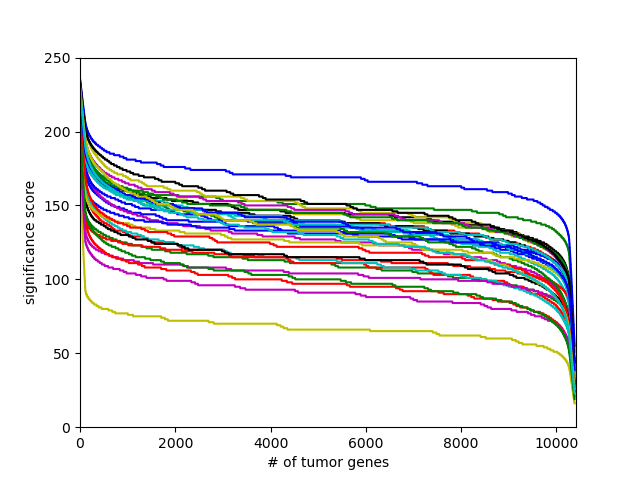
\includegraphics[width=0.7\textwidth]{images/confidence-score/ConfidenceScore-plot-VarNet.png}
    \caption{I cambi di intensità nelle heatmap per ogni classe. Si può notare come alcune classi condividano lo stesso pattern nei cambi di intensità.}
    \label{fig:confidence-score-VarNet}
\end{figure}
Stesso discorso vale per le pathway biologiche rilevate: esse sono del tutto identiche a quelle rilevate a seguito dei
test con la rete Net, così come riportato nella sezione \ref{ssec:val-bio-net}.
Nelle Tabella che segue si utilizzerà la seguente legenda: i valori di questo \textcolor{\clrnew}{colore} sono 
le nuove pathway rilevate dalle nostre analisi con il tool DAVID, i valori con questo \colorbox{\clrmatch}{background}
indicano le path che trovano riscontro anche nel lavoro di Lyu e Haque \cite{lyu2018deep} e i valori con questo
\colorbox{\clrpath}{\textbf{background}} indicano quelle pathway che sono specifiche
della coorte tumorale.

\begin{longtable}{cllr}
%intestazione iniziale
\caption{Risultati della Pathways Analysis sui primi 400 geni per ogni tipo di tumore ($P < 10^{-3}$)} \\
\toprule
\multirow{2}{*}{Tumore} & \multicolumn{2}{l}{Pathway correlata} & \multirow{2}{*}{P value} \\
& ID & Nome \\
\midrule
\endfirsthead
\toprule
\multirow{2}{*}{Tumore} & \multicolumn{2}{l}{Pathway correlata} & \multirow{2}{*}{P value} \\
& ID & Nome \\
\midrule
\endhead
\midrule
\multicolumn{2}{r}{Continua nella prossima pagina}
\endfoot
\bottomrule
\endlastfoot
ACC & hsa04010 & \textcolor{\clrnew}{MAPK signaling pathway} & 2.58e-07\\ 
 & hsa04015 & \textcolor{\clrnew}{Rap1 signaling pathway} & 2.65e-05 \\ 
 & hsa04512 & \textcolor{\clrnew}{ECM-receptor interaction} & 3.77e-05 \\ 
 & hsa04976 & \textcolor{\clrnew}{Bile secretion} & 1.33e-04 \\ 
 & hsa04115 & \textcolor{\clrnew}{p53 signaling pathway} & 3.75e-04 \\ 
 & hsa04610 & \textcolor{\clrnew}{Complement and coagulation cascades} & 5.56e-04 \\ 
 & hsa05144 & \textcolor{\clrnew}{Malaria} & 7.06e-04 \\ 
\midrule 
\rowcolor{\clrmatch}BLCA & hsa04512 & ECM-receptor interaction & 9.98e-08\\ 
 & hsa05205 & \textcolor{\clrnew}{Proteoglycans in cancer} & 2.15e-07 \\ 
 & hsa04514 & \textcolor{\clrnew}{Cell adhesion molecules} & 7.48e-06 \\ 
 \rowcolor{\clrmatch}& hsa04510 & Focal adhesion & 1.01e-05 \\ 
 & hsa05150 & \textcolor{\clrnew}{Staphylococcus aureus infection} & 7.54e-05 \\ 
 & hsa04270 & \textcolor{\clrnew}{Vascular smooth muscle contraction} & 1.26e-04 \\ 
 & hsa04668 & \textcolor{\clrnew}{TNF signaling pathway} & 1.64e-04 \\ 
 & hsa05200 & \textcolor{\clrnew}{Pathways in cancer} & 2.11e-04 \\ 
 & hsa04933 & \textcolor{\clrnew}{AGE-RAGE signaling pathway in diabetic complications} & 4.00e-04 \\ 
 & hsa04913 & \textcolor{\clrnew}{Ovarian steroidogenesis} & 5.06e-04 \\ 
 & hsa05165 & \textcolor{\clrnew}{Human papillomavirus infection} & 9.06e-04 \\ 
 & hsa05166 & \textcolor{\clrnew}{Human T-cell leukemia virus 1 infection} & 9.85e-04 \\ 
\midrule 
BRCA & hsa04915 & \textcolor{\clrnew}{Estrogen signaling pathway} & 2.38e-08\\ 
 \rowcolor{\clrmatch}& hsa04512 & ECM-receptor interaction & 2.44e-08 \\ 
 \rowcolor{\clrpath}& hsa04151 & \textbf{PI3K-Akt signaling pathway *} & 4.61e-06 \\ 
 & hsa04927 & \textcolor{\clrnew}{Cortisol synthesis and secretion} & 8.11e-06 \\ 
 & hsa04928 & \textcolor{\clrnew}{Parathyroid hormone synthesis, secretion and action} & 2.10e-05 \\ 
 & hsa04934 & \textcolor{\clrnew}{Cushing syndrome} & 3.31e-05 \\ 
 \rowcolor{\clrmatch}& hsa04510 & Focal adhesion & 4.96e-05 \\ 
 & hsa05205 & \textcolor{\clrnew}{Proteoglycans in cancer} & 8.05e-05 \\ 
 & hsa05165 & \textcolor{\clrnew}{Human papillomavirus infection} & 8.86e-05 \\ 
 \rowcolor{\clrpath}& hsa03320 & \textbf{PPAR signaling pathway *} & 8.95e-05 \\ 
 & hsa04514 & \textcolor{\clrnew}{Cell adhesion molecules} & 1.03e-04 \\ 
 & hsa04145 & \textcolor{\clrnew}{Phagosome} & 1.20e-04 \\ 
 & hsa04933 & \textcolor{\clrnew}{AGE-RAGE signaling pathway in diabetic complications} & 1.51e-04 \\ 
 & hsa05200 & \textcolor{\clrnew}{Pathways in cancer} & 5.14e-04 \\ 
 & hsa01522 & \textcolor{\clrnew}{Endocrine resistance} & 7.22e-04 \\ 
 & hsa04926 & \textcolor{\clrnew}{Relaxin signaling pathway} & 7.76e-04 \\ 
 & hsa04540 & \textcolor{\clrnew}{Gap junction} & 9.62e-04 \\ 
\midrule 
CESC & hsa05200 & \textcolor{\clrnew}{Pathways in cancer} & 8.37e-07\\ 
 & hsa04115 & \textcolor{\clrnew}{p53 signaling pathway} & 4.64e-06 \\ 
 \rowcolor{\clrpath}& hsa05205 & \textbf{Proteoglycans in cancer} & 5.71e-05 \\ 
 & hsa05222 & \textcolor{\clrnew}{Small cell lung cancer} & 8.00e-05 \\ 
 & hsa04512 & \textcolor{\clrnew}{ECM-receptor interaction} & 1.14e-04 \\ 
 & hsa04110 & \textcolor{\clrnew}{Cell cycle} & 1.54e-04 \\ 
 & hsa05146 & \textcolor{\clrnew}{Amoebiasis} & 1.57e-04 \\ 
 & hsa04080 & \textcolor{\clrnew}{Neuroactive ligand-receptor interaction} & 1.79e-04 \\ 
 & hsa04915 & \textcolor{\clrnew}{Estrogen signaling pathway} & 2.85e-04 \\ 
 & hsa04934 & \textcolor{\clrnew}{Cushing syndrome} & 4.46e-04 \\ 
 & hsa05144 & \textcolor{\clrnew}{Malaria} & 5.78e-04 \\ 
\midrule 
CHOL & hsa04512 & \textcolor{\clrnew}{ECM-receptor interaction} & 3.94e-10\\ 
 & hsa04610 & \textcolor{\clrnew}{Complement and coagulation cascades} & 1.92e-08 \\ 
 & hsa00340 & \textcolor{\clrnew}{Histidine metabolism} & 6.82e-06 \\ 
 & hsa04061 & \textcolor{\clrnew}{Viral protein interaction with cytokine and cytokine receptor} & 8.03e-06 \\ 
 & hsa04514 & \textcolor{\clrnew}{Cell adhesion molecules} & 1.59e-05 \\ 
 & hsa04015 & \textcolor{\clrnew}{Rap1 signaling pathway} & 2.18e-05 \\ 
 & hsa04020 & \textcolor{\clrnew}{Calcium signaling pathway} & 3.36e-05 \\ 
 & hsa04510 & \textcolor{\clrnew}{Focal adhesion} & 3.57e-05 \\ 
 & hsa04974 & \textcolor{\clrnew}{Protein digestion and absorption} & 4.25e-05 \\ 
 & hsa04950 & \textcolor{\clrnew}{Maturity onset diabetes of the young} & 4.90e-05 \\ 
 & hsa04540 & \textcolor{\clrnew}{Gap junction} & 6.49e-05 \\ 
 & hsa04080 & \textcolor{\clrnew}{Neuroactive ligand-receptor interaction} & 8.23e-05 \\ 
 & hsa05146 & \textcolor{\clrnew}{Amoebiasis} & 9.96e-05 \\ 
 & hsa04060 & \textcolor{\clrnew}{Cytokine-cytokine receptor interaction} & 1.37e-04 \\ 
 & hsa04928 & \textcolor{\clrnew}{Parathyroid hormone synthesis, secretion and action} & 1.92e-04 \\ 
 & hsa04062 & \textcolor{\clrnew}{Chemokine signaling pathway} & 2.71e-04 \\ 
 & hsa05414 & \textcolor{\clrnew}{Dilated cardiomyopathy} & 6.96e-04 \\ 
 & hsa04530 & \textcolor{\clrnew}{Tight junction} & 8.58e-04 \\ 
 \rowcolor{\clrpath}& hsa04151 & \textbf{PI3K-Akt signaling pathway **} & 8.82e-04 \\ 
\midrule 
COAD & hsa04640 & \textcolor{\clrnew}{Hematopoietic cell lineage} & 6.01e-06\\ 
 & hsa04145 & \textcolor{\clrnew}{Phagosome} & 1.01e-05 \\ 
 & hsa04060 & \textcolor{\clrnew}{Cytokine-cytokine receptor interaction} & 1.18e-05 \\ 
 & hsa04974 & \textcolor{\clrnew}{Protein digestion and absorption} & 1.37e-05 \\ 
 & hsa04512 & \textcolor{\clrnew}{ECM-receptor interaction} & 1.73e-05 \\ 
 & hsa04080 & \textcolor{\clrnew}{Neuroactive ligand-receptor interaction} & 4.12e-05 \\ 
 & hsa04514 & \textcolor{\clrnew}{Cell adhesion molecules} & 5.28e-05 \\ 
 & hsa05332 & \textcolor{\clrnew}{Graft-versus-host disease} & 1.96e-04 \\ 
 & hsa05323 & \textcolor{\clrnew}{Rheumatoid arthritis} & 9.33e-04 \\ 
\midrule 
\rowcolor{\clrmatch}DLBC & hsa04940 & Type I diabetes mellitus & 7.84e-11\\ 
 \rowcolor{\clrpath}& hsa05330 & \textbf{Allograft rejection} & 1.85e-10 \\ 
 \rowcolor{\clrpath}& hsa05332 & \textbf{Graft-versus-host disease} & 3.28e-10 \\ 
 \rowcolor{\clrmatch}& hsa04640 & Hematopoietic cell lineage & 5.58e-10 \\ 
 & hsa04659 & \textcolor{\clrnew}{Th17 cell differentiation} & 6.90e-10 \\ 
 \rowcolor{\clrmatch}& hsa04672 & Intestinal immune network for IgA production & 2.72e-09 \\ 
 \rowcolor{\clrmatch}& hsa04145 & Phagosome & 2.08e-08 \\ 
 \rowcolor{\clrmatch}& hsa05321 & Inflammatory bowel disease & 2.47e-08 \\ 
 \rowcolor{\clrmatch}& hsa05150 & Staphylococcus aureus infection & 4.84e-08 \\ 
 & hsa04658 & \textcolor{\clrnew}{Th1 and Th2 cell differentiation} & 5.35e-08 \\ 
 \rowcolor{\clrmatch}& hsa05323 & Rheumatoid arthritis & 7.22e-08 \\ 
 \rowcolor{\clrmatch}& hsa05416 & Viral myocarditis & 7.58e-08 \\ 
 \rowcolor{\clrmatch}& hsa05140 & Leishmaniasis & 1.01e-07 \\ 
 & hsa04061 & \textcolor{\clrnew}{Viral protein interaction with cytokine and cytokine receptor} & 1.52e-07 \\ 
 \rowcolor{\clrpath}& hsa04514 & \textbf{Cell adhesion molecules} & 1.78e-07 \\ 
 \rowcolor{\clrmatch}& hsa05320 & Autoimmune thyroid disease & 4.97e-07 \\ 
 & hsa04610 & \textcolor{\clrnew}{Complement and coagulation cascades} & 1.50e-06 \\ 
 \rowcolor{\clrpath}& hsa04062 & \textbf{Chemokine signaling pathway} & 2.65e-06 \\ 
 & hsa05169 & \textcolor{\clrnew}{Epstein-Barr virus infection} & 5.57e-06 \\ 
 \rowcolor{\clrmatch}& hsa05166 & Human T-cell leukemia virus 1 infection & 9.70e-06 \\ 
 \rowcolor{\clrmatch}& hsa04060 & Cytokine-cytokine receptor interaction & 1.04e-05 \\ 
 & hsa05133 & \textcolor{\clrnew}{Pertussis} & 1.29e-05 \\ 
 \rowcolor{\clrpath}& hsa04662 & \textbf{B cell receptor signaling pathway} & 1.83e-05 \\ 
 \rowcolor{\clrmatch}& hsa05310 & Asthma & 1.91e-05 \\ 
 & hsa04380 & \textcolor{\clrnew}{Osteoclast differentiation} & 2.74e-05 \\ 
 \rowcolor{\clrmatch}& hsa05152 & Tuberculosis & 1.20e-04 \\ 
 \rowcolor{\clrmatch}& hsa05145 & Toxoplasmosis & 1.51e-04 \\ 
 \rowcolor{\clrmatch}& hsa04612 & Antigen processing and presentation & 1.89e-04 \\ 
 \rowcolor{\clrpath}& hsa04064 & \textbf{NF-kappa B signaling pathway} & 2.26e-04 \\ 
 & hsa04621 & \textcolor{\clrnew}{NOD-like receptor signaling pathway} & 4.09e-04 \\ 
 & hsa05130 & \textcolor{\clrnew}{Pathogenic Escherichia coli infection} & 4.96e-04 \\ 
 & hsa04115 & \textcolor{\clrnew}{p53 signaling pathway} & 5.14e-04 \\ 
 & hsa04625 & \textcolor{\clrnew}{C-type lectin receptor signaling pathway} & 5.46e-04 \\ 
 & hsa04928 & \textcolor{\clrnew}{Parathyroid hormone synthesis, secretion and action} & 7.52e-04 \\ 
\midrule 
\rowcolor{\clrmatch}ESCA & hsa04512 & ECM-receptor interaction & 1.38e-12\\ 
 & hsa05414 & \textcolor{\clrnew}{Dilated cardiomyopathy} & 5.86e-10 \\ 
 \rowcolor{\clrmatch}& hsa05412 & Arrhythmogenic right ventricular cardiomyopathy & 2.79e-09 \\ 
 \rowcolor{\clrmatch}& hsa04510 & Focal adhesion & 2.85e-08 \\ 
 & hsa05410 & \textcolor{\clrnew}{Hypertrophic cardiomyopathy} & 3.42e-08 \\ 
 & hsa05165 & \textcolor{\clrnew}{Human papillomavirus infection} & 2.32e-07 \\ 
 & hsa05200 & \textcolor{\clrnew}{Pathways in cancer} & 2.31e-06 \\ 
 & hsa04022 & \textcolor{\clrnew}{cGMP-PKG signaling pathway} & 1.55e-05 \\ 
 & hsa04151 & \textcolor{\clrnew}{PI3K-Akt signaling pathway *} & 2.25e-05 \\ 
 & hsa05146 & \textcolor{\clrnew}{Amoebiasis} & 6.56e-05 \\ 
 & hsa05222 & \textcolor{\clrnew}{Small cell lung cancer} & 9.19e-05 \\ 
 & hsa04934 & \textcolor{\clrnew}{Cushing syndrome} & 1.02e-04 \\ 
 & hsa05205 & \textcolor{\clrnew}{Proteoglycans in cancer} & 1.50e-04 \\ 
 & hsa04360 & \textcolor{\clrnew}{Axon guidance} & 2.40e-04 \\ 
 & hsa04550 & \textcolor{\clrnew}{Signaling pathways regulating pluripotency of stem cells} & 2.72e-04 \\ 
 & hsa04390 & \textcolor{\clrnew}{Hippo signaling pathway} & 2.99e-04 \\ 
 & hsa04916 & \textcolor{\clrnew}{Melanogenesis} & 4.06e-04 \\ 
 & hsa02010 & \textcolor{\clrnew}{ABC transporters} & 7.09e-04 \\ 
 & hsa05224 & \textcolor{\clrnew}{Breast cancer} & 9.80e-04 \\ 
\midrule 
GBM & hsa04060 & \textcolor{\clrnew}{Cytokine-cytokine receptor interaction} & 4.80e-10\\ 
 & hsa04080 & \textcolor{\clrnew}{Neuroactive ligand-receptor interaction} & 8.72e-10 \\ 
 & hsa04062 & \textcolor{\clrnew}{Chemokine signaling pathway} & 2.85e-06 \\ 
 & hsa04061 & \textcolor{\clrnew}{Viral protein interaction with cytokine and cytokine receptor} & 7.48e-06 \\ 
 & hsa05323 & \textcolor{\clrnew}{Rheumatoid arthritis} & 1.50e-05 \\ 
 & hsa04015 & \textcolor{\clrnew}{Rap1 signaling pathway} & 3.59e-05 \\ 
 & hsa05205 & \textcolor{\clrnew}{Proteoglycans in cancer} & 4.06e-05 \\ 
 & hsa04512 & \textcolor{\clrnew}{ECM-receptor interaction} & 4.60e-05 \\ 
 & hsa04510 & \textcolor{\clrnew}{Focal adhesion} & 5.20e-05 \\ 
 & hsa05144 & \textcolor{\clrnew}{Malaria} & 6.52e-05 \\ 
 & hsa05032 & \textcolor{\clrnew}{Morphine addiction} & 8.44e-05 \\ 
 & hsa05200 & \textcolor{\clrnew}{Pathways in cancer} & 1.93e-04 \\ 
 & hsa04724 & \textcolor{\clrnew}{Glutamatergic synapse} & 2.69e-04 \\ 
 & hsa04020 & \textcolor{\clrnew}{Calcium signaling pathway} & 5.21e-04 \\ 
 & hsa04974 & \textcolor{\clrnew}{Protein digestion and absorption} & 6.78e-04 \\ 
 \rowcolor{\clrpath}& hsa04151 & \textbf{PI3K-Akt signaling pathway **} & 7.09e-04 \\ 
 & hsa04390 & \textcolor{\clrnew}{Hippo signaling pathway} & 7.86e-04 \\ 
 & hsa04371 & \textcolor{\clrnew}{Apelin signaling pathway} & 7.87e-04 \\ 
 & hsa04270 & \textcolor{\clrnew}{Vascular smooth muscle contraction} & 8.89e-04 \\ 
\midrule 
\rowcolor{\clrmatch}HNSC & hsa04512 & ECM-receptor interaction & 5.74e-12\\ 
 \rowcolor{\clrpath}& hsa05414 & \textbf{Dilated cardiomyopathy} & 8.53e-09 \\ 
 \rowcolor{\clrmatch}& hsa05410 & Hypertrophic cardiomyopathy & 2.73e-08 \\ 
 \rowcolor{\clrmatch}& hsa05412 & Arrhythmogenic right ventricular cardiomyopathy & 2.10e-07 \\ 
 & hsa04510 & \textcolor{\clrnew}{Focal adhesion} & 3.46e-05 \\ 
 & hsa05146 & \textcolor{\clrnew}{Amoebiasis} & 5.55e-05 \\ 
 & hsa04151 & \textcolor{\clrnew}{PI3K-Akt signaling pathway} & 5.93e-05 \\ 
 & hsa04020 & \textcolor{\clrnew}{Calcium signaling pathway} & 6.03e-05 \\ 
 & hsa04713 & \textcolor{\clrnew}{Circadian entrainment} & 6.61e-05 \\ 
 & hsa05165 & \textcolor{\clrnew}{Human papillomavirus infection} & 1.01e-04 \\ 
 & hsa05150 & \textcolor{\clrnew}{Staphylococcus aureus infection} & 1.58e-04 \\ 
 & hsa04915 & \textcolor{\clrnew}{Estrogen signaling pathway} & 2.79e-04 \\ 
 & hsa04060 & \textcolor{\clrnew}{Cytokine-cytokine receptor interaction} & 3.67e-04 \\ 
 & hsa04926 & \textcolor{\clrnew}{Relaxin signaling pathway} & 4.78e-04 \\ 
 & hsa04921 & \textcolor{\clrnew}{Oxytocin signaling pathway} & 8.48e-04 \\ 
 & hsa04724 & \textcolor{\clrnew}{Glutamatergic synapse} & 8.86e-04 \\ 
\midrule 
KICH & hsa05200 & \textcolor{\clrnew}{Pathways in cancer} & 1.25e-06\\ 
 & hsa04940 & \textcolor{\clrnew}{Type I diabetes mellitus} & 6.03e-06 \\ 
 & hsa04015 & \textcolor{\clrnew}{Rap1 signaling pathway} & 1.42e-05 \\ 
 & hsa04510 & \textcolor{\clrnew}{Focal adhesion} & 2.06e-05 \\ 
 & hsa04916 & \textcolor{\clrnew}{Melanogenesis} & 2.42e-05 \\ 
 & hsa04390 & \textcolor{\clrnew}{Hippo signaling pathway} & 2.90e-05 \\ 
 & hsa05205 & \textcolor{\clrnew}{Proteoglycans in cancer} & 3.50e-05 \\ 
 & hsa04512 & \textcolor{\clrnew}{ECM-receptor interaction} & 4.17e-05 \\ 
 & hsa05217 & \textcolor{\clrnew}{Basal cell carcinoma} & 4.29e-05 \\ 
 & hsa04640 & \textcolor{\clrnew}{Hematopoietic cell lineage} & 4.61e-05 \\ 
 & hsa04010 & \textcolor{\clrnew}{MAPK signaling pathway} & 9.56e-05 \\ 
 & hsa04060 & \textcolor{\clrnew}{Cytokine-cytokine receptor interaction} & 1.06e-04 \\ 
 & hsa05226 & \textcolor{\clrnew}{Gastric cancer} & 1.13e-04 \\ 
 & hsa04933 & \textcolor{\clrnew}{AGE-RAGE signaling pathway in diabetic complications} & 1.50e-04 \\ 
 & hsa04310 & \textcolor{\clrnew}{Wnt signaling pathway *} & 1.79e-04 \\ 
 & hsa05225 & \textcolor{\clrnew}{Hepatocellular carcinoma} & 2.96e-04 \\ 
 & hsa04020 & \textcolor{\clrnew}{Calcium signaling pathway} & 4.55e-04 \\ 
 & hsa04934 & \textcolor{\clrnew}{Cushing syndrome} & 5.54e-04 \\ 
 & hsa05321 & \textcolor{\clrnew}{Inflammatory bowel disease} & 6.77e-04 \\ 
 & hsa00410 & \textcolor{\clrnew}{beta-Alanine metabolism} & 8.03e-04 \\ 
 & hsa05224 & \textcolor{\clrnew}{Breast cancer} & 9.13e-04 \\ 
\midrule 
KIRC & hsa04514 & \textcolor{\clrnew}{Cell adhesion molecules} & 5.72e-08\\ 
 & hsa04060 & \textcolor{\clrnew}{Cytokine-cytokine receptor interaction} & 1.70e-07 \\ 
 & hsa04640 & \textcolor{\clrnew}{Hematopoietic cell lineage} & 8.25e-07 \\ 
 & hsa04061 & \textcolor{\clrnew}{Viral protein interaction with cytokine and cytokine receptor} & 3.35e-06 \\ 
 & hsa04512 & \textcolor{\clrnew}{ECM-receptor interaction} & 6.44e-06 \\ 
 \rowcolor{\clrpath}& hsa04610 & \textbf{Complement and coagulation cascades} & 1.28e-05 \\ 
 & hsa05332 & \textcolor{\clrnew}{Graft-versus-host disease} & 1.10e-04 \\ 
 & hsa04510 & \textcolor{\clrnew}{Focal adhesion} & 1.57e-04 \\ 
 & hsa04015 & \textcolor{\clrnew}{Rap1 signaling pathway} & 2.23e-04 \\ 
 & hsa04080 & \textcolor{\clrnew}{Neuroactive ligand-receptor interaction} & 3.87e-04 \\ 
 & hsa04940 & \textcolor{\clrnew}{Type I diabetes mellitus} & 5.56e-04 \\ 
 & hsa04360 & \textcolor{\clrnew}{Axon guidance} & 5.71e-04 \\ 
 & hsa04151 & \textcolor{\clrnew}{PI3K-Akt signaling pathway *} & 6.52e-04 \\ 
 & hsa03320 & \textcolor{\clrnew}{PPAR signaling pathway} & 7.84e-04 \\ 
 & hsa05205 & \textcolor{\clrnew}{Proteoglycans in cancer} & 9.41e-04 \\ 
 & hsa05144 & \textcolor{\clrnew}{Malaria} & 9.42e-04 \\ 
\midrule 
\rowcolor{\clrmatch}KIRP & hsa04512 & ECM-receptor interaction & 7.01e-13\\ 
 & hsa04976 & \textcolor{\clrnew}{Bile secretion} & 1.98e-07 \\ 
 \rowcolor{\clrmatch}& hsa04510 & Focal adhesion & 1.26e-06 \\ 
 \rowcolor{\clrmatch}& hsa04974 & Protein digestion and absorption & 1.82e-06 \\ 
 & hsa05146 & \textcolor{\clrnew}{Amoebiasis} & 4.60e-06 \\ 
 & hsa04360 & \textcolor{\clrnew}{Axon guidance} & 3.32e-05 \\ 
 & hsa04928 & \textcolor{\clrnew}{Parathyroid hormone synthesis, secretion and action} & 8.28e-05 \\ 
 & hsa00260 & \textcolor{\clrnew}{Glycine, serine and threonine metabolism} & 1.22e-04 \\ 
 & hsa02010 & \textcolor{\clrnew}{ABC transporters} & 1.33e-04 \\ 
 & hsa04915 & \textcolor{\clrnew}{Estrogen signaling pathway} & 1.34e-04 \\ 
 & hsa04151 & \textcolor{\clrnew}{PI3K-Akt signaling pathway *} & 3.46e-04 \\ 
 & hsa00053 & \textcolor{\clrnew}{Ascorbate and aldarate metabolism} & 4.11e-04 \\ 
 & hsa04015 & \textcolor{\clrnew}{Rap1 signaling pathway} & 4.43e-04 \\ 
 & hsa04640 & \textcolor{\clrnew}{Hematopoietic cell lineage} & 4.49e-04 \\ 
 & hsa00340 & \textcolor{\clrnew}{Histidine metabolism} & 5.43e-04 \\ 
 & hsa00010 & \textcolor{\clrnew}{Glycolysis / Gluconeogenesis} & 6.20e-04 \\ 
 & hsa00650 & \textcolor{\clrnew}{Butanoate metabolism} & 6.85e-04 \\ 
 & hsa05414 & \textcolor{\clrnew}{Dilated cardiomyopathy} & 7.00e-04 \\ 
 & hsa04514 & \textcolor{\clrnew}{Cell adhesion molecules} & 7.19e-04 \\ 
 & hsa00620 & \textcolor{\clrnew}{Pyruvate metabolism} & 8.10e-04 \\ 
\midrule 
LAML & hsa04640 & \textcolor{\clrnew}{Hematopoietic cell lineage} & 1.99e-15\\ 
 & hsa05200 & \textcolor{\clrnew}{Pathways in cancer} & 3.52e-08 \\ 
 \rowcolor{\clrpath}& hsa05140 & \textbf{Leishmaniasis} & 3.95e-08 \\ 
 & hsa04380 & \textcolor{\clrnew}{Osteoclast differentiation} & 5.34e-08 \\ 
 & hsa04514 & \textcolor{\clrnew}{Cell adhesion molecules} & 3.93e-07 \\ 
 & hsa05321 & \textcolor{\clrnew}{Inflammatory bowel disease} & 8.93e-07 \\ 
 & hsa05143 & \textcolor{\clrnew}{African trypanosomiasis} & 9.97e-07 \\ 
 & hsa05332 & \textcolor{\clrnew}{Graft-versus-host disease} & 1.69e-06 \\ 
 & hsa05340 & \textcolor{\clrnew}{Primary immunodeficiency} & 8.45e-06 \\ 
 & hsa04940 & \textcolor{\clrnew}{Type I diabetes mellitus} & 1.22e-05 \\ 
 & hsa04060 & \textcolor{\clrnew}{Cytokine-cytokine receptor interaction} & 1.97e-05 \\ 
 & hsa05414 & \textcolor{\clrnew}{Dilated cardiomyopathy} & 2.26e-05 \\ 
 & hsa04658 & \textcolor{\clrnew}{Th1 and Th2 cell differentiation} & 2.79e-05 \\ 
 & hsa04062 & \textcolor{\clrnew}{Chemokine signaling pathway} & 4.92e-05 \\ 
 & hsa04061 & \textcolor{\clrnew}{Viral protein interaction with cytokine and cytokine receptor} & 5.12e-05 \\ 
 & hsa05310 & \textcolor{\clrnew}{Asthma} & 6.28e-05 \\ 
 & hsa04970 & \textcolor{\clrnew}{Salivary secretion} & 7.93e-05 \\ 
 & hsa04659 & \textcolor{\clrnew}{Th17 cell differentiation} & 8.71e-05 \\ 
 \rowcolor{\clrpath}& hsa04672 & \textbf{Intestinal immune network for IgA production} & 8.74e-05 \\ 
 & hsa05323 & \textcolor{\clrnew}{Rheumatoid arthritis} & 9.67e-05 \\ 
 & hsa04015 & \textcolor{\clrnew}{Rap1 signaling pathway} & 1.13e-04 \\ 
 & hsa04072 & \textcolor{\clrnew}{Phospholipase D signaling pathway} & 1.24e-04 \\ 
 & hsa04933 & \textcolor{\clrnew}{AGE-RAGE signaling pathway in diabetic complications} & 1.37e-04 \\ 
 & hsa05150 & \textcolor{\clrnew}{Staphylococcus aureus infection} & 1.71e-04 \\ 
 & hsa05330 & \textcolor{\clrnew}{Allograft rejection} & 1.76e-04 \\ 
 & hsa04611 & \textcolor{\clrnew}{Platelet activation} & 2.12e-04 \\ 
 & hsa04145 & \textcolor{\clrnew}{Phagosome} & 2.19e-04 \\ 
 & hsa04010 & \textcolor{\clrnew}{MAPK signaling pathway} & 2.19e-04 \\ 
 & hsa04670 & \textcolor{\clrnew}{Leukocyte transendothelial migration} & 2.43e-04 \\ 
 & hsa04750 & \textcolor{\clrnew}{Inflammatory mediator regulation of TRP channels} & 2.45e-04 \\ 
 & hsa05410 & \textcolor{\clrnew}{Hypertrophic cardiomyopathy} & 3.87e-04 \\ 
 & hsa05144 & \textcolor{\clrnew}{Malaria} & 4.05e-04 \\ 
 & hsa04662 & \textcolor{\clrnew}{B cell receptor signaling pathway} & 6.09e-04 \\ 
 & hsa04625 & \textcolor{\clrnew}{C-type lectin receptor signaling pathway} & 6.67e-04 \\ 
 & hsa05418 & \textcolor{\clrnew}{Fluid shear stress and atherosclerosis} & 8.10e-04 \\ 
\midrule 
LGG & hsa04512 & \textcolor{\clrnew}{ECM-receptor interaction} & 2.13e-06\\ 
 & hsa04510 & \textcolor{\clrnew}{Focal adhesion} & 3.42e-06 \\ 
 & hsa04974 & \textcolor{\clrnew}{Protein digestion and absorption} & 1.83e-05 \\ 
 & hsa04640 & \textcolor{\clrnew}{Hematopoietic cell lineage} & 2.42e-05 \\ 
 & hsa04015 & \textcolor{\clrnew}{Rap1 signaling pathway} & 1.20e-04 \\ 
 & hsa04020 & \textcolor{\clrnew}{Calcium signaling pathway} & 1.96e-04 \\ 
 & hsa04724 & \textcolor{\clrnew}{Glutamatergic synapse} & 3.25e-04 \\ 
 \rowcolor{\clrpath}& hsa04010 & \textbf{MAPK signaling pathway **} & 4.16e-04 \\ 
 & hsa04145 & \textcolor{\clrnew}{Phagosome} & 4.22e-04 \\ 
 & hsa02010 & \textcolor{\clrnew}{ABC transporters} & 5.18e-04 \\ 
 & hsa04972 & \textcolor{\clrnew}{Pancreatic secretion} & 7.57e-04 \\ 
 & hsa04080 & \textcolor{\clrnew}{Neuroactive ligand-receptor interaction} & 9.97e-04 \\ 
\midrule 
\rowcolor{\clrmatch}LIHC & hsa04610 & Complement and coagulation cascades & 2.48e-15\\ 
 & hsa05150 & \textcolor{\clrnew}{Staphylococcus aureus infection} & 1.08e-08 \\ 
 & hsa03320 & \textcolor{\clrnew}{PPAR signaling pathway} & 3.42e-06 \\ 
 & hsa04216 & \textcolor{\clrnew}{Ferroptosis} & 4.49e-06 \\ 
 & hsa04979 & \textcolor{\clrnew}{Cholesterol metabolism} & 8.20e-06 \\ 
 & hsa04940 & \textcolor{\clrnew}{Type I diabetes mellitus} & 9.71e-06 \\ 
 & hsa00140 & \textcolor{\clrnew}{Steroid hormone biosynthesis} & 1.55e-05 \\ 
 & hsa04950 & \textcolor{\clrnew}{Maturity onset diabetes of the young} & 3.21e-05 \\ 
 & hsa04514 & \textcolor{\clrnew}{Cell adhesion molecules} & 6.27e-05 \\ 
 & hsa05332 & \textcolor{\clrnew}{Graft-versus-host disease} & 1.28e-04 \\ 
 & hsa05330 & \textcolor{\clrnew}{Allograft rejection} & 1.46e-04 \\ 
 & hsa05323 & \textcolor{\clrnew}{Rheumatoid arthritis} & 1.97e-04 \\ 
 & hsa04612 & \textcolor{\clrnew}{Antigen processing and presentation} & 2.22e-04 \\ 
 \rowcolor{\clrmatch}& hsa00830 & Retinol metabolism & 2.29e-04 \\ 
 & hsa04061 & \textcolor{\clrnew}{Viral protein interaction with cytokine and cytokine receptor} & 2.65e-04 \\ 
 \rowcolor{\clrpath}& hsa04060 & \textbf{Cytokine-cytokine receptor interaction **} & 2.74e-04 \\ 
 \rowcolor{\clrpath}& hsa04062 & \textbf{Chemokine signaling pathway **} & 2.99e-04 \\ 
 & hsa05321 & \textcolor{\clrnew}{Inflammatory bowel disease} & 3.57e-04 \\ 
\midrule 
LUAD & hsa04610 & \textcolor{\clrnew}{Complement and coagulation cascades} & 1.82e-07\\ 
 & hsa04145 & \textcolor{\clrnew}{Phagosome} & 4.00e-06 \\ 
 & hsa04514 & \textcolor{\clrnew}{Cell adhesion molecules} & 5.46e-05 \\ 
 & hsa05150 & \textcolor{\clrnew}{Staphylococcus aureus infection} & 6.39e-05 \\ 
 & hsa05205 & \textcolor{\clrnew}{Proteoglycans in cancer} & 3.05e-04 \\ 
 & hsa05416 & \textcolor{\clrnew}{Viral myocarditis} & 4.79e-04 \\ 
\midrule 
LUSC & hsa04512 & \textcolor{\clrnew}{ECM-receptor interaction} & 1.39e-08\\ 
 & hsa04060 & \textcolor{\clrnew}{Cytokine-cytokine receptor interaction} & 1.81e-07 \\ 
 & hsa04061 & \textcolor{\clrnew}{Viral protein interaction with cytokine and cytokine receptor} & 3.53e-07 \\ 
 & hsa04514 & \textcolor{\clrnew}{Cell adhesion molecules} & 4.09e-06 \\ 
 & hsa04640 & \textcolor{\clrnew}{Hematopoietic cell lineage} & 3.00e-05 \\ 
 & hsa04976 & \textcolor{\clrnew}{Bile secretion} & 1.11e-04 \\ 
 \rowcolor{\clrpath}& hsa04151 & \textbf{PI3K-Akt signaling pathway **} & 3.13e-04 \\ 
 & hsa05200 & \textcolor{\clrnew}{Pathways in cancer} & 3.68e-04 \\ 
 & hsa04610 & \textcolor{\clrnew}{Complement and coagulation cascades} & 5.04e-04 \\ 
\midrule 
\rowcolor{\clrmatch}MESO & hsa04610 & Complement and coagulation cascades & 2.56e-09\\ 
 & hsa04080 & \textcolor{\clrnew}{Neuroactive ligand-receptor interaction} & 1.26e-07 \\ 
 \rowcolor{\clrmatch}& hsa04512 & ECM-receptor interaction & 3.08e-07 \\ 
 & hsa05144 & \textcolor{\clrnew}{Malaria} & 6.56e-07 \\ 
 \rowcolor{\clrpath}& hsa05150 & \textbf{Staphylococcus aureus infection} & 7.07e-07 \\ 
 & hsa04020 & \textcolor{\clrnew}{Calcium signaling pathway} & 5.55e-06 \\ 
 \rowcolor{\clrmatch}& hsa04974 & Protein digestion and absorption & 3.15e-05 \\ 
 \rowcolor{\clrmatch}& hsa04510 & Focal adhesion & 3.79e-05 \\ 
 & hsa05205 & \textcolor{\clrnew}{Proteoglycans in cancer} & 1.31e-04 \\ 
 & hsa04390 & \textcolor{\clrnew}{Hippo signaling pathway} & 1.33e-04 \\ 
 & hsa04514 & \textcolor{\clrnew}{Cell adhesion molecules} & 1.33e-04 \\ 
 & hsa04061 & \textcolor{\clrnew}{Viral protein interaction with cytokine and cytokine receptor} & 1.34e-04 \\ 
 \rowcolor{\clrmatch}& hsa04145 & Phagosome & 1.51e-04 \\ 
 & hsa04915 & \textcolor{\clrnew}{Estrogen signaling pathway} & 2.49e-04 \\ 
 & hsa04621 & \textcolor{\clrnew}{NOD-like receptor signaling pathway} & 4.07e-04 \\ 
 & hsa05030 & \textcolor{\clrnew}{Cocaine addiction} & 5.50e-04 \\ 
 & hsa05165 & \textcolor{\clrnew}{Human papillomavirus infection} & 6.73e-04 \\ 
 & hsa05033 & \textcolor{\clrnew}{Nicotine addiction} & 6.76e-04 \\ 
 & hsa04015 & \textcolor{\clrnew}{Rap1 signaling pathway} & 8.79e-04 \\ 
 & hsa04060 & \textcolor{\clrnew}{Cytokine-cytokine receptor interaction} & 9.22e-04 \\ 
 & hsa04350 & \textcolor{\clrnew}{TGF-beta signaling pathway} & 9.52e-04 \\ 
\midrule 
OV & hsa04360 & \textcolor{\clrnew}{Axon guidance} & 1.30e-05\\ 
 & hsa04514 & \textcolor{\clrnew}{Cell adhesion molecules} & 2.59e-05 \\ 
 & hsa05200 & \textcolor{\clrnew}{Pathways in cancer} & 1.34e-04 \\ 
 & hsa05205 & \textcolor{\clrnew}{Proteoglycans in cancer} & 9.19e-04 \\ 
\midrule 
\rowcolor{\clrmatch}PAAD & hsa04974 & Protein digestion and absorption & 6.26e-11\\ 
 \rowcolor{\clrmatch}& hsa04512 & ECM-receptor interaction & 4.23e-08 \\ 
 & hsa04080 & \textcolor{\clrnew}{Neuroactive ligand-receptor interaction} & 2.22e-07 \\ 
 & hsa04972 & \textcolor{\clrnew}{Pancreatic secretion} & 5.47e-07 \\ 
 \rowcolor{\clrmatch}& hsa04950 & Maturity onset diabetes of the young & 5.65e-07 \\ 
 & hsa04610 & \textcolor{\clrnew}{Complement and coagulation cascades} & 1.21e-06 \\ 
 & hsa04510 & \textcolor{\clrnew}{Focal adhesion} & 7.62e-06 \\ 
 & hsa05414 & \textcolor{\clrnew}{Dilated cardiomyopathy} & 3.86e-05 \\ 
 & hsa04024 & \textcolor{\clrnew}{cAMP signaling pathway} & 5.05e-05 \\ 
 & hsa04911 & \textcolor{\clrnew}{Insulin secretion} & 1.17e-04 \\ 
 & hsa04670 & \textcolor{\clrnew}{Leukocyte transendothelial migration} & 3.59e-04 \\ 
 & hsa04060 & \textcolor{\clrnew}{Cytokine-cytokine receptor interaction} & 3.62e-04 \\ 
 & hsa04015 & \textcolor{\clrnew}{Rap1 signaling pathway} & 4.55e-04 \\ 
 & hsa04976 & \textcolor{\clrnew}{Bile secretion} & 5.47e-04 \\ 
 & hsa04978 & \textcolor{\clrnew}{Mineral absorption} & 9.30e-04 \\ 
\midrule 
PCPG & hsa04510 & \textcolor{\clrnew}{Focal adhesion} & 3.73e-07\\ 
 & hsa04514 & \textcolor{\clrnew}{Cell adhesion molecules} & 7.34e-07 \\ 
 & hsa04933 & \textcolor{\clrnew}{AGE-RAGE signaling pathway in diabetic complications} & 1.42e-05 \\ 
 & hsa04512 & \textcolor{\clrnew}{ECM-receptor interaction} & 2.73e-05 \\ 
 & hsa05205 & \textcolor{\clrnew}{Proteoglycans in cancer} & 4.34e-05 \\ 
 \rowcolor{\clrpath}& hsa04010 & \textbf{MAPK signaling pathway **} & 4.36e-05 \\ 
 & hsa04940 & \textcolor{\clrnew}{Type I diabetes mellitus} & 4.52e-05 \\ 
 & hsa05200 & \textcolor{\clrnew}{Pathways in cancer} & 5.98e-05 \\ 
 & hsa05416 & \textcolor{\clrnew}{Viral myocarditis} & 1.17e-04 \\ 
 & hsa04080 & \textcolor{\clrnew}{Neuroactive ligand-receptor interaction} & 1.27e-04 \\ 
 & hsa05332 & \textcolor{\clrnew}{Graft-versus-host disease} & 1.34e-04 \\ 
 & hsa05145 & \textcolor{\clrnew}{Toxoplasmosis} & 1.39e-04 \\ 
 & hsa05032 & \textcolor{\clrnew}{Morphine addiction} & 1.44e-04 \\ 
 & hsa04062 & \textcolor{\clrnew}{Chemokine signaling pathway} & 1.60e-04 \\ 
 & hsa04727 & \textcolor{\clrnew}{GABAergic synapse} & 2.64e-04 \\ 
 & hsa04060 & \textcolor{\clrnew}{Cytokine-cytokine receptor interaction} & 3.03e-04 \\ 
 & hsa04926 & \textcolor{\clrnew}{Relaxin signaling pathway} & 3.55e-04 \\ 
 & hsa04145 & \textcolor{\clrnew}{Phagosome} & 3.66e-04 \\ 
 & hsa04610 & \textcolor{\clrnew}{Complement and coagulation cascades} & 4.01e-04 \\ 
 & hsa04724 & \textcolor{\clrnew}{Glutamatergic synapse} & 4.62e-04 \\ 
 & hsa04925 & \textcolor{\clrnew}{Aldosterone synthesis and secretion} & 5.00e-04 \\ 
 & hsa04020 & \textcolor{\clrnew}{Calcium signaling pathway} & 5.94e-04 \\ 
 & hsa05330 & \textcolor{\clrnew}{Allograft rejection} & 6.02e-04 \\ 
 \rowcolor{\clrpath}& hsa04151 & \textbf{PI3K-Akt signaling pathway **} & 6.18e-04 \\ 
 & hsa04612 & \textcolor{\clrnew}{Antigen processing and presentation} & 6.42e-04 \\ 
 & hsa05410 & \textcolor{\clrnew}{Hypertrophic cardiomyopathy} & 8.04e-04 \\ 
 & hsa05414 & \textcolor{\clrnew}{Dilated cardiomyopathy} & 8.77e-04 \\ 
\midrule 
PRAD & hsa04514 & \textcolor{\clrnew}{Cell adhesion molecules} & 1.12e-08\\ 
 & hsa05205 & \textcolor{\clrnew}{Proteoglycans in cancer} & 2.34e-05 \\ 
 & hsa04940 & \textcolor{\clrnew}{Type I diabetes mellitus} & 6.91e-05 \\ 
 & hsa04061 & \textcolor{\clrnew}{Viral protein interaction with cytokine and cytokine receptor} & 7.51e-05 \\ 
 & hsa04010 & \textcolor{\clrnew}{MAPK signaling pathway} & 2.19e-04 \\ 
 & hsa04060 & \textcolor{\clrnew}{Cytokine-cytokine receptor interaction} & 2.41e-04 \\ 
 \rowcolor{\clrpath}& hsa04270 & \textbf{Vascular smooth muscle contraction} & 2.72e-04 \\ 
 & hsa04640 & \textcolor{\clrnew}{Hematopoietic cell lineage} & 4.10e-04 \\ 
 & hsa02010 & \textcolor{\clrnew}{ABC transporters} & 4.70e-04 \\ 
 & hsa05150 & \textcolor{\clrnew}{Staphylococcus aureus infection} & 6.03e-04 \\ 
 & hsa05130 & \textcolor{\clrnew}{Pathogenic Escherichia coli infection} & 6.11e-04 \\ 
\midrule 
READ & hsa04080 & \textcolor{\clrnew}{Neuroactive ligand-receptor interaction} & 9.20e-09\\ 
 & hsa04514 & \textcolor{\clrnew}{Cell adhesion molecules} & 1.60e-07 \\ 
 & hsa04510 & \textcolor{\clrnew}{Focal adhesion} & 1.28e-06 \\ 
 & hsa05146 & \textcolor{\clrnew}{Amoebiasis} & 1.66e-06 \\ 
 & hsa04060 & \textcolor{\clrnew}{Cytokine-cytokine receptor interaction} & 1.67e-06 \\ 
 & hsa04512 & \textcolor{\clrnew}{ECM-receptor interaction} & 1.92e-06 \\ 
 & hsa04015 & \textcolor{\clrnew}{Rap1 signaling pathway} & 2.16e-06 \\ 
 & hsa04020 & \textcolor{\clrnew}{Calcium signaling pathway} & 1.06e-04 \\ 
 & hsa04014 & \textcolor{\clrnew}{Ras signaling pathway} & 1.33e-04 \\ 
 & hsa04061 & \textcolor{\clrnew}{Viral protein interaction with cytokine and cytokine receptor} & 2.10e-04 \\ 
 & hsa05032 & \textcolor{\clrnew}{Morphine addiction} & 2.88e-04 \\ 
 & hsa05200 & \textcolor{\clrnew}{Pathways in cancer} & 3.21e-04 \\ 
 & hsa04270 & \textcolor{\clrnew}{Vascular smooth muscle contraction} & 5.22e-04 \\ 
 & hsa04611 & \textcolor{\clrnew}{Platelet activation} & 6.47e-04 \\ 
 & hsa04610 & \textcolor{\clrnew}{Complement and coagulation cascades} & 7.99e-04 \\ 
 & hsa05205 & \textcolor{\clrnew}{Proteoglycans in cancer} & 9.23e-04 \\ 
 & hsa05144 & \textcolor{\clrnew}{Malaria} & 9.32e-04 \\ 
\midrule 
\rowcolor{\clrmatch}SARC & hsa04512 & ECM-receptor interaction & 9.92e-08\\ 
 & hsa05205 & \textcolor{\clrnew}{Proteoglycans in cancer} & 1.33e-06 \\ 
 & hsa05410 & \textcolor{\clrnew}{Hypertrophic cardiomyopathy} & 2.26e-06 \\ 
 \rowcolor{\clrmatch}& hsa04510 & Focal adhesion & 4.53e-06 \\ 
 & hsa05414 & \textcolor{\clrnew}{Dilated cardiomyopathy} & 2.60e-05 \\ 
 & hsa04514 & \textcolor{\clrnew}{Cell adhesion molecules} & 2.83e-05 \\ 
 \rowcolor{\clrmatch}& hsa04151 & PI3K-Akt signaling pathway & 1.08e-04 \\ 
 & hsa05200 & \textcolor{\clrnew}{Pathways in cancer} & 1.64e-04 \\ 
 & hsa04020 & \textcolor{\clrnew}{Calcium signaling pathway} & 1.98e-04 \\ 
 & hsa04610 & \textcolor{\clrnew}{Complement and coagulation cascades} & 3.00e-04 \\ 
 & hsa05416 & \textcolor{\clrnew}{Viral myocarditis} & 5.43e-04 \\ 
 \rowcolor{\clrmatch}& hsa04974 & Protein digestion and absorption & 6.30e-04 \\ 
 & hsa05144 & \textcolor{\clrnew}{Malaria} & 7.01e-04 \\ 
\midrule 
\rowcolor{\clrmatch}SKCM & hsa04512 & ECM-receptor interaction & 2.05e-09\\ 
 & hsa04514 & \textcolor{\clrnew}{Cell adhesion molecules} & 1.05e-06 \\ 
 \rowcolor{\clrmatch}& hsa04510 & Focal adhesion & 1.40e-05 \\ 
 \rowcolor{\clrmatch}& hsa04974 & Protein digestion and absorption & 4.75e-05 \\ 
 & hsa04970 & \textcolor{\clrnew}{Salivary secretion} & 1.20e-04 \\ 
 & hsa04145 & \textcolor{\clrnew}{Phagosome} & 2.35e-04 \\ 
 & hsa04360 & \textcolor{\clrnew}{Axon guidance} & 2.50e-04 \\ 
 & hsa04640 & \textcolor{\clrnew}{Hematopoietic cell lineage} & 4.15e-04 \\ 
 & hsa05205 & \textcolor{\clrnew}{Proteoglycans in cancer} & 4.35e-04 \\ 
 & hsa04061 & \textcolor{\clrnew}{Viral protein interaction with cytokine and cytokine receptor} & 4.89e-04 \\ 
 & hsa04062 & \textcolor{\clrnew}{Chemokine signaling pathway} & 7.83e-04 \\ 
 & hsa05416 & \textcolor{\clrnew}{Viral myocarditis} & 8.52e-04 \\ 
 & hsa05202 & \textcolor{\clrnew}{Transcriptional misregulation in cancer} & 8.72e-04 \\ 
\midrule 
STAD & hsa04080 & \textcolor{\clrnew}{Neuroactive ligand-receptor interaction} & 1.29e-07\\ 
 & hsa04060 & \textcolor{\clrnew}{Cytokine-cytokine receptor interaction} & 1.70e-05 \\ 
 & hsa04020 & \textcolor{\clrnew}{Calcium signaling pathway} & 5.87e-04 \\ 
\midrule 
TGCT & hsa04514 & \textcolor{\clrnew}{Cell adhesion molecules} & 5.25e-07\\ 
 & hsa04940 & \textcolor{\clrnew}{Type I diabetes mellitus} & 5.73e-07 \\ 
 & hsa05410 & \textcolor{\clrnew}{Hypertrophic cardiomyopathy} & 6.61e-07 \\ 
 \rowcolor{\clrmatch}& hsa04512 & ECM-receptor interaction & 1.32e-06 \\ 
 & hsa05414 & \textcolor{\clrnew}{Dilated cardiomyopathy} & 3.05e-06 \\ 
 & hsa05412 & \textcolor{\clrnew}{Arrhythmogenic right ventricular cardiomyopathy} & 9.50e-06 \\ 
 \rowcolor{\clrmatch}& hsa04974 & Protein digestion and absorption & 1.47e-05 \\ 
 & hsa05416 & \textcolor{\clrnew}{Viral myocarditis} & 4.79e-05 \\ 
 & hsa05205 & \textcolor{\clrnew}{Proteoglycans in cancer} & 7.82e-05 \\ 
 & hsa04510 & \textcolor{\clrnew}{Focal adhesion} & 9.72e-05 \\ 
 & hsa04145 & \textcolor{\clrnew}{Phagosome} & 1.22e-04 \\ 
 & hsa04061 & \textcolor{\clrnew}{Viral protein interaction with cytokine and cytokine receptor} & 1.62e-04 \\ 
 & hsa05332 & \textcolor{\clrnew}{Graft-versus-host disease} & 1.75e-04 \\ 
 & hsa05130 & \textcolor{\clrnew}{Pathogenic Escherichia coli infection} & 2.45e-04 \\ 
 & hsa04540 & \textcolor{\clrnew}{Gap junction} & 3.13e-04 \\ 
 & hsa04261 & \textcolor{\clrnew}{Adrenergic signaling in cardiomyocytes} & 4.38e-04 \\ 
 & hsa04062 & \textcolor{\clrnew}{Chemokine signaling pathway} & 5.34e-04 \\ 
 & hsa05330 & \textcolor{\clrnew}{Allograft rejection} & 7.56e-04 \\ 
 & hsa04550 & \textcolor{\clrnew}{Signaling pathways regulating pluripotency of stem cells} & 7.75e-04 \\ 
 & hsa04975 & \textcolor{\clrnew}{Fat digestion and absorption} & 8.41e-04 \\ 
\midrule 
THCA & hsa04514 & \textcolor{\clrnew}{Cell adhesion molecules} & 3.21e-08\\ 
 \rowcolor{\clrmatch}& hsa04512 & ECM-receptor interaction & 1.32e-07 \\ 
 \rowcolor{\clrmatch}& hsa04510 & Focal adhesion & 5.79e-06 \\ 
 & hsa05205 & \textcolor{\clrnew}{Proteoglycans in cancer} & 1.00e-04 \\ 
 & hsa05146 & \textcolor{\clrnew}{Amoebiasis} & 1.08e-04 \\ 
 & hsa05144 & \textcolor{\clrnew}{Malaria} & 1.50e-04 \\ 
 & hsa04933 & \textcolor{\clrnew}{AGE-RAGE signaling pathway in diabetic complications} & 1.93e-04 \\ 
 & hsa05410 & \textcolor{\clrnew}{Hypertrophic cardiomyopathy} & 2.03e-04 \\ 
 & hsa04151 & \textcolor{\clrnew}{PI3K-Akt signaling pathway} & 3.40e-04 \\ 
 & hsa05200 & \textcolor{\clrnew}{Pathways in cancer} & 3.41e-04 \\ 
 & hsa04670 & \textcolor{\clrnew}{Leukocyte transendothelial migration} & 3.45e-04 \\ 
 & hsa04020 & \textcolor{\clrnew}{Calcium signaling pathway} & 3.83e-04 \\ 
\midrule 
THYM & hsa04514 & \textcolor{\clrnew}{Cell adhesion molecules} & 5.87e-10\\ 
 & hsa04672 & \textcolor{\clrnew}{Intestinal immune network for IgA production} & 1.43e-08 \\ 
 & hsa05150 & \textcolor{\clrnew}{Staphylococcus aureus infection} & 4.04e-08 \\ 
 \rowcolor{\clrmatch}& hsa04640 & Hematopoietic cell lineage & 3.30e-07 \\ 
 & hsa04940 & \textcolor{\clrnew}{Type I diabetes mellitus} & 4.25e-06 \\ 
 & hsa05416 & \textcolor{\clrnew}{Viral myocarditis} & 5.22e-06 \\ 
 & hsa04145 & \textcolor{\clrnew}{Phagosome} & 6.94e-06 \\ 
 & hsa04658 & \textcolor{\clrnew}{Th1 and Th2 cell differentiation} & 1.82e-05 \\ 
 & hsa05321 & \textcolor{\clrnew}{Inflammatory bowel disease} & 2.28e-05 \\ 
 & hsa04612 & \textcolor{\clrnew}{Antigen processing and presentation} & 5.83e-05 \\ 
 & hsa05332 & \textcolor{\clrnew}{Graft-versus-host disease} & 5.86e-05 \\ 
 & hsa05323 & \textcolor{\clrnew}{Rheumatoid arthritis} & 6.42e-05 \\ 
 & hsa04015 & \textcolor{\clrnew}{Rap1 signaling pathway} & 1.32e-04 \\ 
 & hsa05412 & \textcolor{\clrnew}{Arrhythmogenic right ventricular cardiomyopathy} & 1.37e-04 \\ 
 & hsa04659 & \textcolor{\clrnew}{Th17 cell differentiation} & 1.63e-04 \\ 
 & hsa04810 & \textcolor{\clrnew}{Regulation of actin cytoskeleton} & 1.65e-04 \\ 
 & hsa04512 & \textcolor{\clrnew}{ECM-receptor interaction} & 1.74e-04 \\ 
 & hsa05330 & \textcolor{\clrnew}{Allograft rejection} & 2.56e-04 \\ 
 & hsa04510 & \textcolor{\clrnew}{Focal adhesion} & 3.46e-04 \\ 
 & hsa04060 & \textcolor{\clrnew}{Cytokine-cytokine receptor interaction} & 6.09e-04 \\ 
 & hsa04151 & \textcolor{\clrnew}{PI3K-Akt signaling pathway} & 8.45e-04 \\ 
 \rowcolor{\clrpath}& hsa05340 & \textbf{Primary immunodeficiency} & 9.58e-04 \\ 
 & hsa04020 & \textcolor{\clrnew}{Calcium signaling pathway} & 9.76e-04 \\ 
\midrule 
UCEC & hsa05205 & \textcolor{\clrnew}{Proteoglycans in cancer} & 1.59e-06\\ 
 & hsa04670 & \textcolor{\clrnew}{Leukocyte transendothelial migration} & 2.05e-05 \\ 
 \rowcolor{\clrpath}& hsa04530 & \textbf{Tight junction} & 5.91e-05 \\ 
 & hsa04020 & \textcolor{\clrnew}{Calcium signaling pathway} & 6.01e-05 \\ 
 & hsa04514 & \textcolor{\clrnew}{Cell adhesion molecules} & 6.29e-05 \\ 
 & hsa04940 & \textcolor{\clrnew}{Type I diabetes mellitus} & 1.84e-04 \\ 
 & hsa05230 & \textcolor{\clrnew}{Central carbon metabolism in cancer} & 2.17e-04 \\ 
 & hsa05200 & \textcolor{\clrnew}{Pathways in cancer} & 2.29e-04 \\ 
 & hsa04512 & \textcolor{\clrnew}{ECM-receptor interaction} & 2.62e-04 \\ 
 & hsa05416 & \textcolor{\clrnew}{Viral myocarditis} & 2.64e-04 \\ 
 & hsa04611 & \textcolor{\clrnew}{Platelet activation} & 2.65e-04 \\ 
 & hsa05165 & \textcolor{\clrnew}{Human papillomavirus infection} & 2.71e-04 \\ 
 & hsa05145 & \textcolor{\clrnew}{Toxoplasmosis} & 2.73e-04 \\ 
 & hsa05332 & \textcolor{\clrnew}{Graft-versus-host disease} & 5.42e-04 \\ 
 & hsa04360 & \textcolor{\clrnew}{Axon guidance} & 6.07e-04 \\ 
 & hsa04550 & \textcolor{\clrnew}{Signaling pathways regulating pluripotency of stem cells} & 6.19e-04 \\ 
 & hsa05130 & \textcolor{\clrnew}{Pathogenic Escherichia coli infection} & 7.20e-04 \\ 
 & hsa05140 & \textcolor{\clrnew}{Leishmaniasis} & 8.01e-04 \\ 
 & hsa05418 & \textcolor{\clrnew}{Fluid shear stress and atherosclerosis} & 8.32e-04 \\ 
 & hsa04659 & \textcolor{\clrnew}{Th17 cell differentiation} & 9.04e-04 \\ 
 & hsa05414 & \textcolor{\clrnew}{Dilated cardiomyopathy} & 9.47e-04 \\ 
 & hsa04612 & \textcolor{\clrnew}{Antigen processing and presentation} & 9.48e-04 \\ 
 & hsa04270 & \textcolor{\clrnew}{Vascular smooth muscle contraction} & 9.90e-04 \\ 
\midrule 
\rowcolor{\clrmatch}UCS & hsa04512 & ECM-receptor interaction & 2.44e-08\\ 
 & hsa05410 & \textcolor{\clrnew}{Hypertrophic cardiomyopathy} & 6.86e-06 \\ 
 & hsa04360 & \textcolor{\clrnew}{Axon guidance} & 1.67e-05 \\ 
 & hsa04080 & \textcolor{\clrnew}{Neuroactive ligand-receptor interaction} & 1.98e-05 \\ 
 \rowcolor{\clrmatch}& hsa04974 & Protein digestion and absorption & 3.58e-05 \\ 
 & hsa05414 & \textcolor{\clrnew}{Dilated cardiomyopathy} & 7.21e-05 \\ 
 & hsa05412 & \textcolor{\clrnew}{Arrhythmogenic right ventricular cardiomyopathy} & 1.08e-04 \\ 
 & hsa05205 & \textcolor{\clrnew}{Proteoglycans in cancer} & 1.54e-04 \\ 
 & hsa05200 & \textcolor{\clrnew}{Pathways in cancer} & 1.57e-04 \\ 
 \rowcolor{\clrmatch}& hsa04510 & Focal adhesion & 1.97e-04 \\ 
 & hsa04151 & \textcolor{\clrnew}{PI3K-Akt signaling pathway} & 2.06e-04 \\ 
 & hsa04145 & \textcolor{\clrnew}{Phagosome} & 3.79e-04 \\ 
 & hsa04550 & \textcolor{\clrnew}{Signaling pathways regulating pluripotency of stem cells} & 5.53e-04 \\ 
 & hsa05165 & \textcolor{\clrnew}{Human papillomavirus infection} & 8.07e-04 \\ 
 & hsa04024 & \textcolor{\clrnew}{cAMP signaling pathway} & 8.55e-04 \\ 
 & hsa04010 & \textcolor{\clrnew}{MAPK signaling pathway} & 9.99e-04 \\ 
\midrule 
UVM & hsa04940 & \textcolor{\clrnew}{Type I diabetes mellitus} & 4.06e-05\\ 
 & hsa04540 & \textcolor{\clrnew}{Gap junction} & 6.89e-05 \\ 
 & hsa05145 & \textcolor{\clrnew}{Toxoplasmosis} & 1.19e-04 \\ 
 \rowcolor{\clrpath}& hsa04010 & MAPK signaling pathway ** & 1.20e-04 \\ 
 & hsa05032 & \textcolor{\clrnew}{Morphine addiction} & 1.25e-04 \\ 
 & hsa04020 & \textcolor{\clrnew}{Calcium signaling pathway} & 1.35e-04 \\ 
 & hsa04530 & \textcolor{\clrnew}{Tight junction} & 1.37e-04 \\ 
 & hsa04974 & \textcolor{\clrnew}{Protein digestion and absorption} & 1.62e-04 \\ 
 & hsa04510 & \textcolor{\clrnew}{Focal adhesion} & 1.91e-04 \\ 
 & hsa04512 & \textcolor{\clrnew}{ECM-receptor interaction} & 1.92e-04 \\ 
 & hsa04916 & \textcolor{\clrnew}{Melanogenesis} & 2.91e-04 \\ 
 & hsa05414 & \textcolor{\clrnew}{Dilated cardiomyopathy} & 3.12e-04 \\ 
 & hsa05140 & \textcolor{\clrnew}{Leishmaniasis} & 4.74e-04 \\ 
 & hsa05330 & \textcolor{\clrnew}{Allograft rejection} & 5.54e-04 \\ 
 & hsa04612 & \textcolor{\clrnew}{Antigen processing and presentation} & 5.72e-04 \\ 
 & hsa05165 & \textcolor{\clrnew}{Human papillomavirus infection} & 6.13e-04 \\ 
 & hsa04145 & \textcolor{\clrnew}{Phagosome} & 6.59e-04 \\ 
 & hsa04970 & \textcolor{\clrnew}{Salivary secretion} & 9.90e-04 \\ 
\midrule 
\end{longtable} 
